\documentclass{article}
\usepackage{graphicx}
\usepackage{amsmath}
\usepackage{amssymb}
\usepackage{subfigure}
\usepackage{epstopdf}
\usepackage{setspace}
\onehalfspacing
\epstopdfsetup{update} % only regenerate pdf files when eps file is newer
\title{Tuning plasmon of gold nanorods by KCN etching}
\author{Aquiles Carattino \and Saumya Khatua \and Michel
Orrit}

\begin{document}
\maketitle
\abstract{This is the abstract}

\section{Introduction}
In recent years gold nanoparticles received a great amount of attention because
of their size-dependent optical properties \cite{Zijlstra2011}. Gold
nanoparticles have shown to be suitable for a range of experiments and
applications extending from solar cells production \cite{Catchpole2008} to
biosensing \cite{Zijlstra2012}, photodynamic therapy \cite{Zhao2014},
plasmon-enhanced spectroscopies \cite{Sivapalan2013}, bioimaging
\cite{VandenBroek2013}, etc. and they can also be used as building blocks for
bigger nanostructures \cite{Ivanov2011} \cite{Do2013} \cite{Guffey2011}. These
versatility is mainly given by the presence of a collective oscillation of
conduction electrons known as surface plasmon; for the case of gold nanorods
(AuNR) its resonance energy (SPR) depends on the aspect ratio (AR) of the
particle and can be found between $2.3\,\textrm{eV}$ for spheres (AR of $1$) to
even below $0.8\,\textrm{eV}$ for very elongated particles (i.e. they can cover
almost the entire visible spectrum and near infrared.)

Controlling the resonance of the particles is useful when is needed to have
control over the spectral properties of these structures. In almost all the
applications cited above, the SPR is critical for a successful experiment.
Moreover, it may just be needed to have a particle with a resonance coinciding
with the available lasers; or the control over the spectral response of the
particles can be used for generating narrow transparency windows
\cite{Biswas2013}. It was also shown, for instance, that Surface Enhanced Raman
Spectroscopy (SERS) depends highly the plasmon resonance of the particles
employed \cite{Sivapalan2013}. In any case this is only a short list to
highlight the importance of the position of the SPR peak.

One of characteristic that makes gold nanorods versatile is the easiness with
which the resonance peak can be tuned. Usually this is done at the moment of
synthesis \cite{Gou2005}, by controlling the concentrations of growth and seed
solutions it is possible to induce the formation of longer or shorter particles
\cite{Nikoobakht2003}. This methods, however, always present a dispersion in the
size distribution of the outcome, hindering the repeatability and the ability to
build larger, periodic structures.

It is therefore useful a method that allows the in-\textit{situ} control of the
plasmon resonance. This work shows that is possible to change the plasmon
resonance peak in more than $300\,\textrm{meV}$ without degrading the optical
properties (i.e. the FWHM of the peak.) For doing so it is employed KCN as an
etching agent; a known and well understood compound that is used not only in the
nano-industry but also at bigger scales, for instance for gold mining. It's
overall reaction formula is:
\begin{equation*}
4\textrm{Au} + 8\textrm{KCN}^-+\textrm{O}_2 + 2\textrm{H}_2\textrm{O}
\leftrightarrows 4K\textrm{Au(CN)}_2^-+4\textrm{KOH}^-
\end{equation*}
In bulk this compound was used for reducing the aspect ratio of rods, i.e.
blue shifting their plasmon \cite{Jana2002}. In a more recent paper it was also
used for generating highly spherical particles with a narrow size
distribution \cite{Lee2013}.

In this work the opposite trend is observed. Single-particle experiments of the
AuNR immersed in KCN show a red-shift of the plasmon meaning an increase in
their aspect ratio. This is confirmed by tracking the luminescence spectra of
individual rods over time as well as by acquiring SEM images of them. A simple
model where etching is considered as being isotropic and constant (i.e. both the
radius of the particle and it's length diminish at the same rate over time),
yields a good agreement with both sets of experiments.

\section{Experimental method}
The luminescence spectra of single gold nanorods (AuNR) is acquired in a home
built confocal microscope using an Acton 500i Spectrometer. A $532\,\textrm{nm}$
laser is used for exciting the particles with a power in the back focal plane of
of the objective of $300\,\mu\textrm{W}$. A high NA objective (Olympus $60$X NA
$1.4$ Oil immersion) is used for both focusing the laser and collecting the
luminescence. A $532\,\textrm{nm}$ notch filter cuts out the excitation light.

The samples are prepared by spin casting a suspension of AuNR on clean
coverslips and thoroughly rinsing them  with Milli-Q water for eliminating the
excess of CTAB. The samples are then placed in a flowcell; the initial spectra
are taken with the rods immersed in Milli-Q water. This characterization allows
to discard, for instance, clusters of rods. After this, a solution of KCN is
flowed into the cell with concentrations ranging from $3\mu\textrm{M}$ to
$50\mu\textrm{M}$. Then the spectra of approximately $10$ different particles is
acquired consecutively after focusing in each one. The time resolution varies
according to the exposure time and number of particles; in this work a spectra
is taken at least every minute.

For confirming the shape of the particles after the dissolution in KCN, SEM
images are acquired. The samples are prepared by letting a droplet of a
suspension of AuNR dry on top of a silicon wafer and then thoroughly rinsing
them with Milli-Q water for eliminating the excess of CTAB. The same samples are
employed for taking images before and after immersing the particles in
$30\mu\textrm{M}$ KCN. For the analysis only the rods separated from each other
are considered as to reproduce the conditions found in the optical experiment.
After immersing the samples in KCN for a given period of time, they are rinsed
with water to stop the reaction and dried with a nitrogen flow.

Bulk extinction spectra of the suspension of rods used previously is acquired as
a function of time after a solution of KCN is added into the vial. This allows
to compare single-particle experiments with previous results. 

\section{Results}

\begin{figure}[p]
 \centering
 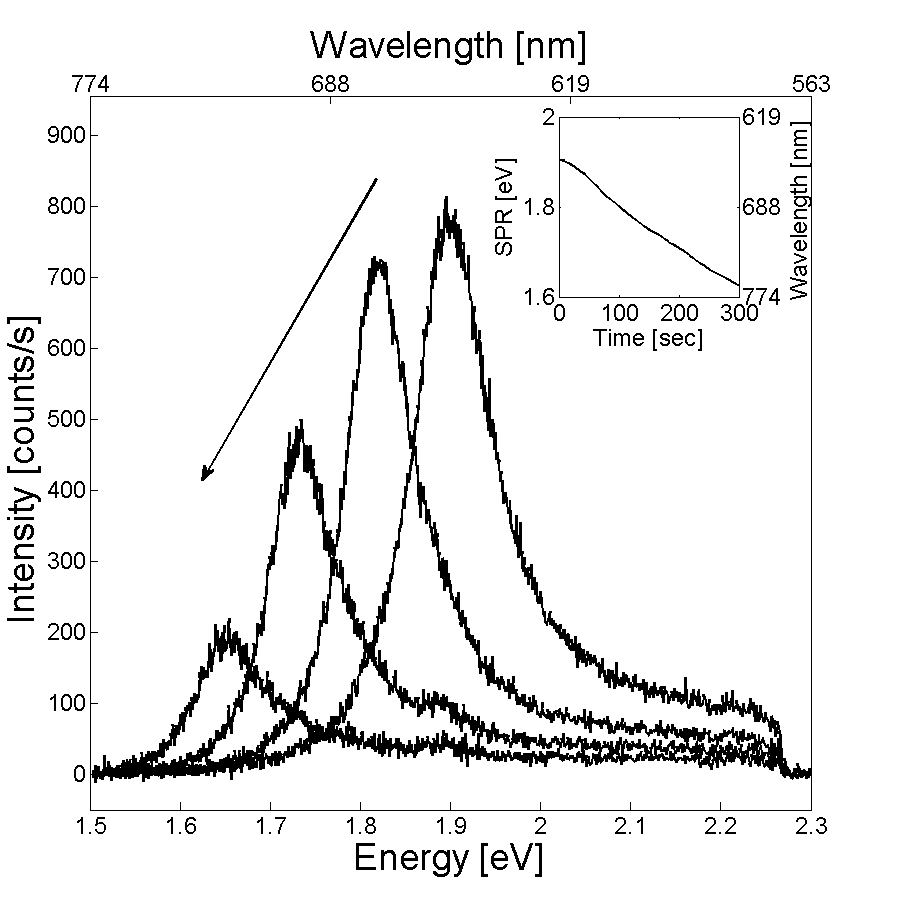
\includegraphics[width=0.95\linewidth]{plasmon_single_rod.png}
 \caption{Plasmon shift due to the etching with $30\mu M$ KCN. The time
 interval between peaks is $70s$. The inset shows the peak position of the SPR as a
 function of time, extracted by fitting the spectra with a lorenzian.}
 \label{fig:plasmon_single_rod}
\end{figure}

Figure \ref{fig:plasmon_single_rod} shows the typical red-shift of the
longitudinal plasmon of a single rod while immersed in $20\,\mu\textrm{M}$ KCN.
Each curve is the luminescence spectra of the same rod displayed at intervals of
$70\,s$ between each other; the small shoulder at $1.9\,\textrm{eV}$
($650\,\textrm{nm}$) that can be observed for the less intense curves is due to
Raman scattering of water that was not completely removed when subtracting the
background to these curves. The inset shows the peak position (calculated by
fitting the spectra with a lorentzian) over time. The plasmon red-shifts over
$0.25\,\textrm{eV}$ ($100\,\textrm{nm}$) in $5$ minutes. This same trend is
observed for all the rods in the same conditions.

\begin{figure}[p]
 \centering
 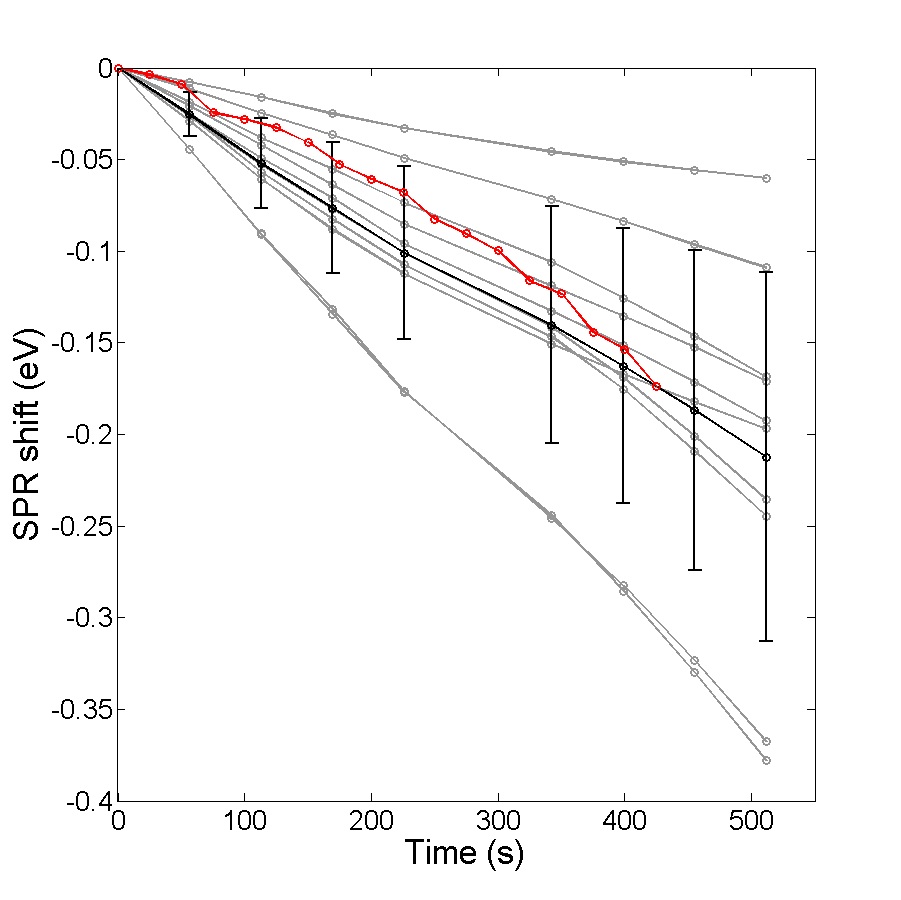
\includegraphics[width=0.95\linewidth]{plasmon_average.png}
 \caption{Average plasmon shift (thick line) for 9 rods due to the etching with
 $30\mu M$ KCN. The light curves are individual time traces while the thick one
 is the average. The error bars are simply the standard deviation at each point. Over
 time the peak distribution gets broader.}
 \label{fig:plasmon_average}
\end{figure}

Figure \ref{fig:plasmon_average} shows the behaviour of the plasmon peak
position for nine different rods while being etched with $20\,\mu\textrm{M}$
KCN. The pale lines show each individual trace, while the darker is the average.
The error bars are the standard deviation of the distribution at each point.
Since spectra of different particles are taken at slightly different times (one
after the other), an interpolation with cubic splines is used for calculating
the average and the standard deviation at the given times. The bigger time step
between $225\,\textrm{s}$ and $340\,\textrm{s}$ is due to an automatic
refocusing happening on the particles every $5$ minutes. The plasmon shift of
each particle ranges between $0.05\,\textrm{eV}$ and $0.35\,\textrm{eV}$ in over
$9 minutes$. It is important to note that the shape of the particles is
preserved during the experiment; the FWHM of each peak is related to the optical
quality of the particles and therefore to their shape.

\begin{figure}[p]
 \centering
 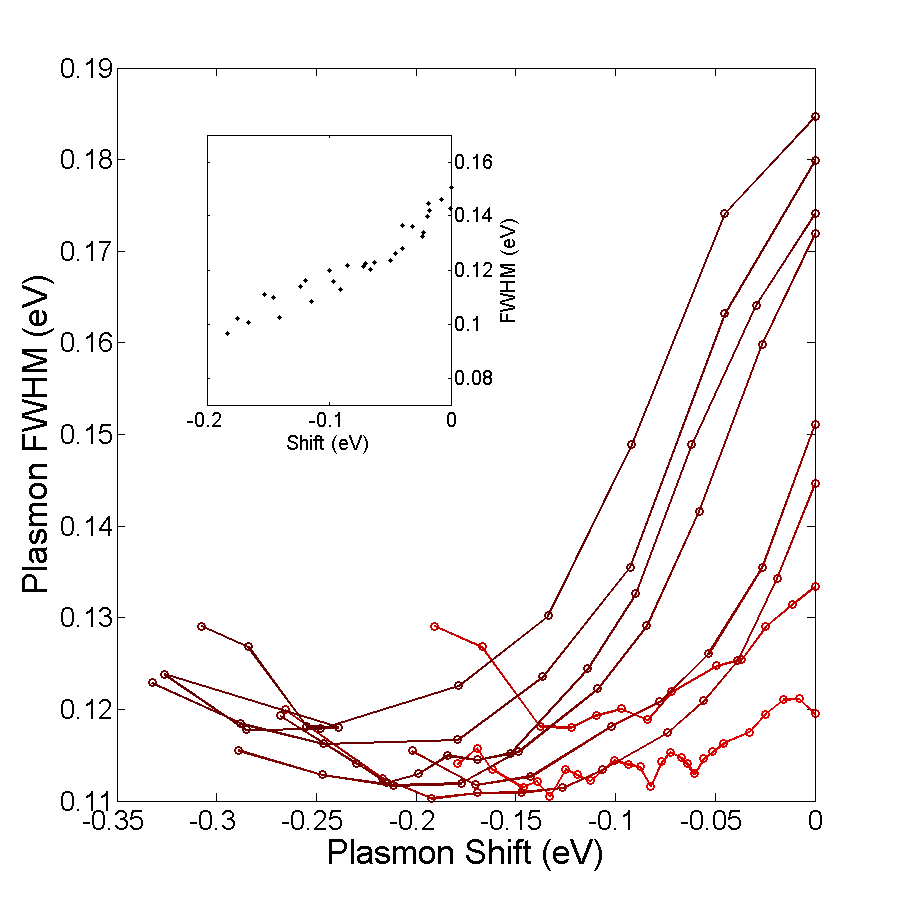
\includegraphics[width=0.95\linewidth]{fwhm_several_in_eV.png}
 \caption{Plasmon FWHM of eight different particles immersed in $20\,\mu M$ KCN
 as a function of their plasmon shift. The inset shows the results from the
 simulations carried on with the ADDA package.}
 \label{fig:FWHM}
\end{figure}


Figure \ref{fig:FWHM} shows that the FWHM of the plasmon decreases while the
shift increases. At the beginning there is a rapid diminishing of the width,
probably due to the elimination of impurities on the surface of the particles.
Then a minimum is reached for shifts between $0.15\,\textrm{eV}$ and
$0.20\,\textrm{eV}$. This decrease is explainable thinking that the higher 
energy distance between the longitudinal plasmon peak and interband transitions
in gold makes less efficient the non radiative damping mechanisms in the
particles, hence yielding a narrower resonance and was already observed in
other studies\cite{Sonnichsen2002}. While the reaction continues, the width
starts to increase; this means that the reshaping at some point will start having an
effect on the shape of the particle. This is often encountered for shifts above
$0.15\,textrm{eV}$, but depends on the particle initial size and shape. ADDA
simulations allow to confirm that the reshaping of the particles induces a
change of the width of the plasmon.


The peak positions are extracted from the simulations in the same way than for
the experiments, by fitting with a lorentzian. Simulations are performed for an
initial $25\times60$ nanoparticle in steps of $0.5\,\textrm{nm}$ for a total of
$10\textrm{nm}$ (i.e. the minimum particle size is $15\textrm{nm}\times 50
\textrm{nm}$). The results are displayed as the red curve in Figure
\ref{fig:plasmon_average} and as the inset in Figure \ref{fig:FWHM}. The best
approximation to the average is found when the etching rate is set to
$1\,\textrm{nm}/min$. This can be further confirmed by SEM images of the rods.
The study of the FWHM of the peak allows to confirm that during this process the
optical properties of the plasmon do not get dampened.
The red curve in the Figure is the result of the simulations that best
fit the experimental results.

The inset in Figure \ref{fig:FWHM} shows the results of the
ADDA\cite{Yurkin2011} simulations for a $25x60$nm particle while both its axis
diminish evenly. The initial FWHM is $0.14\,textrm{eV}$, slightly lower
than the experimentally obtainable. This is due to particles not having a
perfect rod shape, or defects in their crystalline structure. The calculated
width however diminishes to $0.1\,\textrm{eV}$ for shifts of just under
$0.2\,\textrm{eV}$ as it is observed experimentally. This is already showing an
agreement between a model of isotropic etching and our experimental results, and
can also be compared to the plasmon peak shift of different particles.

Samples of the same nanorods are prepared for SEM imaging as described earlier.
The images are acquired before the etching, after $2\,\textrm{min}$ submersed in
KCN and after $4\,\textrm{min}$. When particles are isolated from each other,
the model of the isotropic etching seems appropriate, as the shape is preserved.
It has to be noted, however, that for aggregates of particles this no longer
holds, and rods start to loose their shape (see Supporting Information for SEM
images.) Calculating the distribution of sizes of the particles shows a slight
increase in the aspect ratio but this is however obscured by the broad
distribution of values (even before starting the etching). Averaging around
$300$ different particles at each interval yields an etching constant of
$0.5\,\textrm{nm}/\min$, consistent with the optical observations, not only of
the plasmon shift but also of the diminishing intensity as a function of time. 

It is a known result that the cross section of the particle is proportional to
its volume. Therefore a reduction of size will yield a reduction in intensity
as is observed in all the performed experiments and simulations. Considering an
atomic radius of gold of $144\,\textrm{pm}$(From Wikipedia. Better source?) the
findings show an etching rate of $6000$ atoms per second. On the other hand, a
concentration of $30\mu M$ means that there is roughly $1$ molecule of KCN in a
$1\,\textrm{nm}$ layer of solution around the rod. Is this diffusion limited? 

The same behaviour is observed for rods immersed in different concentrations of
KCN, a red shift that can be of up to $100\,\textrm{nm}$. However the rate at
which the plasmon shifts is different for different particles, as can already be
seen in Figure \ref{fig:plasmon_average}. It is expected that bigger particles
show a slower plasmon shift since the aspect ratio changes more slowly when
reducing the axis length. For instance, a reduction of $1\,\textrm{nm}$ for a
particle with axis $12.5\textrm{nm}\times30\textrm{nm}$ changes the aspect ratio
from  $2.40$ to $2.52$, while for a $25\textrm{nm}\times60\textrm{nm}$ the shift
is to $2.46$. However there is no correlation between the initial brightness
(proportional to the volume) and the observed rate. Different initial aspect
ratios may also show different rates, but again no correlation is observed. This
means that there is an intrinsic property of the particles that makes them react
slower or faster with KCN. This is also confirmed by SEM images, since the
distribution of longitudinal and transverse axis get broader over time.

Every particle can be slightly different from another, not only because of its
aspect ratio (and plasmon peak position) but also because of the presence of
surface impurities. This was shown already in Figure \ref{fig:FWHM} where the
FWHM decreases steeply at the beginning. This implies that different particles
will have slightly different reaction rates, and moreover the effect on the
plasmon may be greater, explaining the different shift-rates. All this
observations at the single-particle level prove to be of fundamental importance 
since they differ from the counterpart bulk experiments. 

\begin{figure}[p]
 \centering 
 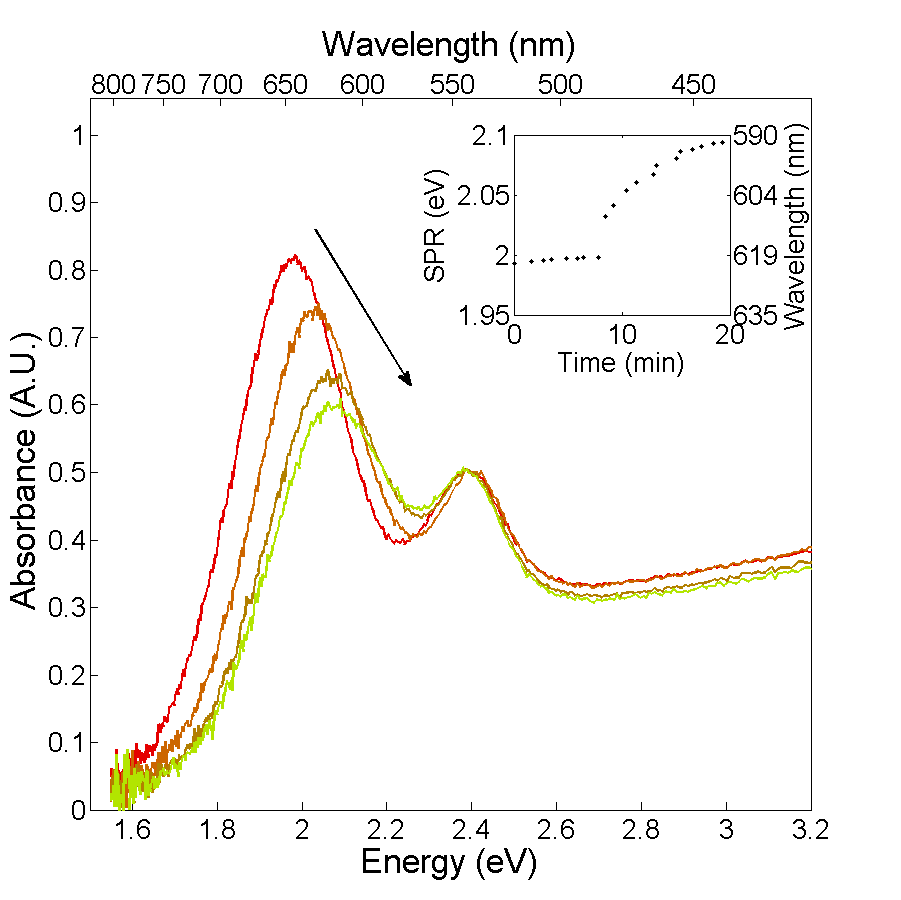
\includegraphics[width=0.95\linewidth]{plasmon_bulk.png}
 \caption{Bulk extinction spectra at $10$ minutes time-interval. The arrow
 indicates the time evolution. A solution of KCN is added into the cuvette with
 the nanorod suspension as to have a $50\,\mu M$ concentration for the first 9
 minutes; then this step is repeated, yielding a final KCN concentration of
 $100\, \mu M$. The inset shows the peak position of the SPR position as a
 function of time, extracted by fitting the spectra with a lorentzian.  }
 \label{fig:bulk}
\end{figure}

Figure \ref{fig:bulk} shows a blue-shift of the longitudinal plasmon peak for a
suspension of rods while being etched with KCN. The spectra is plotted at
intervals of $9$ minutes after adding a solution of KCN. This solution is chosen
as to have $100\mu\textrm{M}$. All spectra plots are normalized to the
transverse plasmon peak at $2.4\,\textrm{eV}$ for increasing the visibility of
the longitudinal plasmon shift. This results are strikingly different from the
single-particle measurements and can be explained by the protective layer of
CTAB present. 

It can be seen that the plasmon peak position shifts towards higher energies
(from approximately $2.0\,\textrm{eV}$ to $2.1\,\textrm{eV}$ or equivalently
from $620\,\textrm{nm}$ to $592\,\textrm{nm}$). It means that the rods are
reshaping into spheres as was previously observed \cite{Jana2002}. This implies
that the tips of the rods are more exposed to KCN than the sides as is expected
from the their higher curvature. The CTAB capping is known to be more dense on
the sides of the particles than on the tips allowing KCN molecules to reach this
region easier. The asymptotic behavior of the time-trace is due to the small
amount of KCN added into the vial, that reacts entirely with gold therefore
stopping the effect after a certain time and can be resumed if added more KCN
into the vial.

The presence of the surface is another aspect that may explain the difference
between the bulk and single-particle results. The surface would prevent the
reaction of gold with KCN from happening on one of the sides of the rods. By
definition this implies a non-isotropic model. On the other hand it would imply
that the shape of the rods is not preserved since they would get flattened. If
this would be the case, the FWHM of the rods is expected to increase and this
work shows that it is not the case, at least for the first couple
hundreds $\textrm{meV}$ of shift. The resolution of SEM images does not allow to
assess this question. The overlap between simulations and experiment gives
enough confidence in the first even if far fetched at first sight.

\begin{figure}[p]
 \centering
 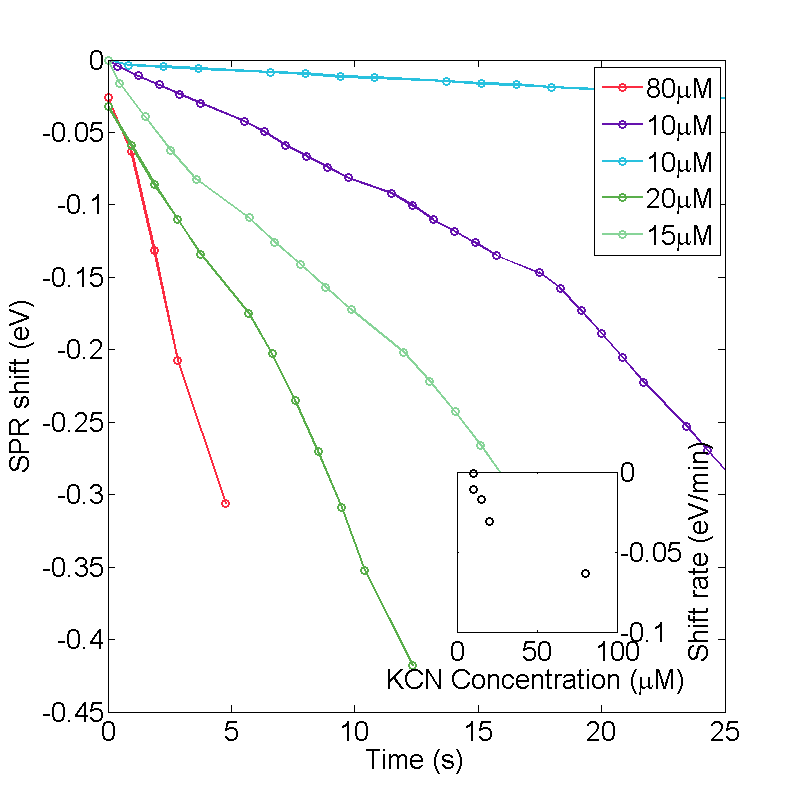
\includegraphics[width=0.95\linewidth]{shift_different_concentrations.png}
 \caption{Plasmon shift of particles with a similar SPR peak at different
 concentrations of KCN as a function of time.}
 \label{fig:FWHM}
\end{figure}

\begin{figure}[p]
 \centering
 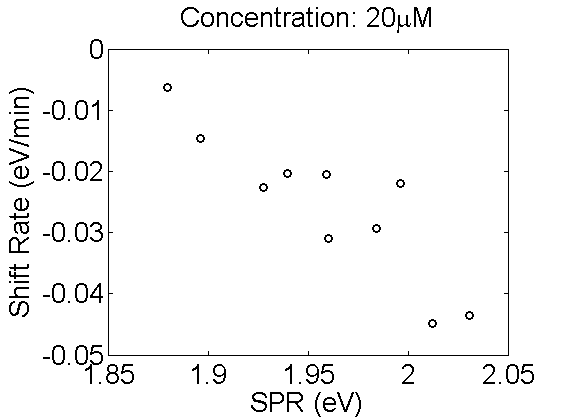
\includegraphics[width=0.95\linewidth]{shift_rate_vs_spr.png}
 \caption{Plasmon shift rate of particles with different initial plasmon peak
 positions when immersed in $20\muM$ KCN.}
 \label{fig:FWHM}
\end{figure}


\section{Conclusions}
In this work we have shown a simple method that allows the tuning of the plasmon
peak position of single gold nanorods with nanometer accuracy and over the range
of $300\,\textrm{meV}$ ($100\,\textrm{nm}$). More importantly, it is shown that
the rodlike shape is preserved for these shifts and therefore the well known
optical properties of the nano particles are not dampened. 

Th experiments allow to acquire plasmon peak with high time and spectral
accuracy, allowing to stop the reaction when the peak is at the desired value.
Both SEM images and the study of the FWHM of the longitudinal resonance allow to
confirm that the shape of the rods is being preserved. The agreement between the
simulations assuming an isotropic etching and the experimental results not only
show the link between both measurements but also provide a way of predicting the
behaviour of the plasmon peak. 

It is also found a great distribution of the rate at which the plasmon peak
shifts for different particles under the same experimental conditions. This can
be explained only considering that there is an intrinsic difference between
particles; this differences can be attributed to defects on the particle surface
or to inhomogeneities in the left over CTAB capping the rods even if care is
taken to remove it by rinsing with water. Different initial conditions (such as
initial aspect ratio or volume) are considered but no correlation with the rate
of the shift is observed. This doesn't discard any relationship between them as
there can be an interwined dependence on both initial size and aspect ratio.
Experiments on larger ensembles of particles would increase the possibility of
finding more nanorods with the same initial conditions. 

Combining this results with the catalytic properties of gold and the presence of
the plasmon resonance opens the door for fine-controlling chemical reactions
while irradiating the particles with specific wavelengths. Using a molecule with
a lower reactivity with gold allows to compare the difference of reaction rates
while exciting or not the longitudinal plasmon. On the other hand this same
technique can be used for detecting the presence of KCN in a solution. This
result was already reported by Wei et Al. in 2012 \cite{Wei2012} in a slightly
different condition. We believe that the sensitivity of single particles to very
low concentrations (in the order or below the nM) should be higher. 

\bibliography{bibliography}{}
\bibliographystyle{ieeetr}

\end{document}
